\documentclass{article}
\usepackage[margin=1in]{geometry}
\usepackage{amsmath,amsthm,amssymb}
\usepackage{bbm,enumerate,mathtools}
\usepackage{tikz,pgfplots}
\usepackage{chessboard}
\usepackage[hidelinks]{hyperref}
\usepackage{multicol} % Problem 35
\usepackage{xstring} % Difficulty command
\usetikzlibrary{shapes.geometric}

\newenvironment{question}{\begin{trivlist}\item[\textbf{Question.}]}{\end{trivlist}}
\newenvironment{note}{\begin{trivlist}\item[\textbf{Note.}]}{\end{trivlist}}
\newenvironment{references}{\begin{trivlist}\item[\textbf{References.}]}{\end{trivlist}}
\newenvironment{related}{\begin{trivlist}\item[\textbf{Related.}]\end{trivlist}\begin{enumerate}}{\end{enumerate}}

\newcommand\score[1]{
\pgfmathsetmacro\pgfxa{#1+1}
\tikzstyle{scorestars}=[
  star,
  star points=5,
  star point ratio=2.25,
  draw,
  inner sep=3pt,
  anchor=outer point 5
]
  \begin{tikzpicture}[baseline]
    \draw[opacity=0] (0,-0.5) rectangle (0,0.2); % Workaround for whitespace at the bottom.
    \foreach \i in {1,...,4} {
      \pgfmathparse{(\i<=#1?"yellow":"gray")}
      \edef\starcolor{\pgfmathresult}
      \draw (\i*4.5ex,0) node[name=star\i,scorestars,fill=\starcolor]  {};
    }
  \end{tikzpicture}
}

\newcommand{\difficulty}[1]{%
  \IfEqCase{#1}{%
      {1}{
        
\begin{tikzpicture}[scale=0.7, baseline=0.9mm]%
          \definecolor{slopegreen}{rgb}{0.0, 0.5, 0.0}%
          \fill[slopegreen] (0.5,0.5) circle (0.5);%
        \end{tikzpicture}%
      }%
      {2}{
        
\begin{tikzpicture}[scale=0.7, baseline=0.9mm]%
          \definecolor{slopeblue}{rgb}{0.0, 0.44, 1.00}
          \fill[slopeblue] (0,0) rectangle (1,1);%
        \end{tikzpicture}%
      }%
      {3}{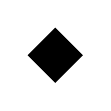
\begin{tikzpicture}[scale=0.7, baseline=0.9mm]\fill (0,0.5)--(0.5, 0)--(1,0.5)--(0.5,1)--cycle; \end{tikzpicture}}%
      {4}{
\begin{tikzpicture}[scale=0.7, baseline=0.9mm]\fill (0.25,0)--(0,0.5)--(0.25,1)--(0.5,0.5)--cycle; \fill (0.75,0)--(0.5,0.5)--(0.75,1)--(1,0.5)--cycle;\end{tikzpicture}}%
      % you can add more cases here as desired
  }[\PackageError{difficulty}{Undefined difficulty level: #1}{}]%
}%
\newcommand{\rating}[2]{\difficulty{#1}\\\score{#2}\\}


\begin{document}
\rating{3}{2}
A Heronian $2$-simplex (triangle) is a triangle with both integer sides and
integer area. A Heronian $n$-simplex is an $n$-simplex with integer volume and
where all sides are Heronian $(n - 1)$-simplices.
\begin{figure}[ht!]
  \centering
  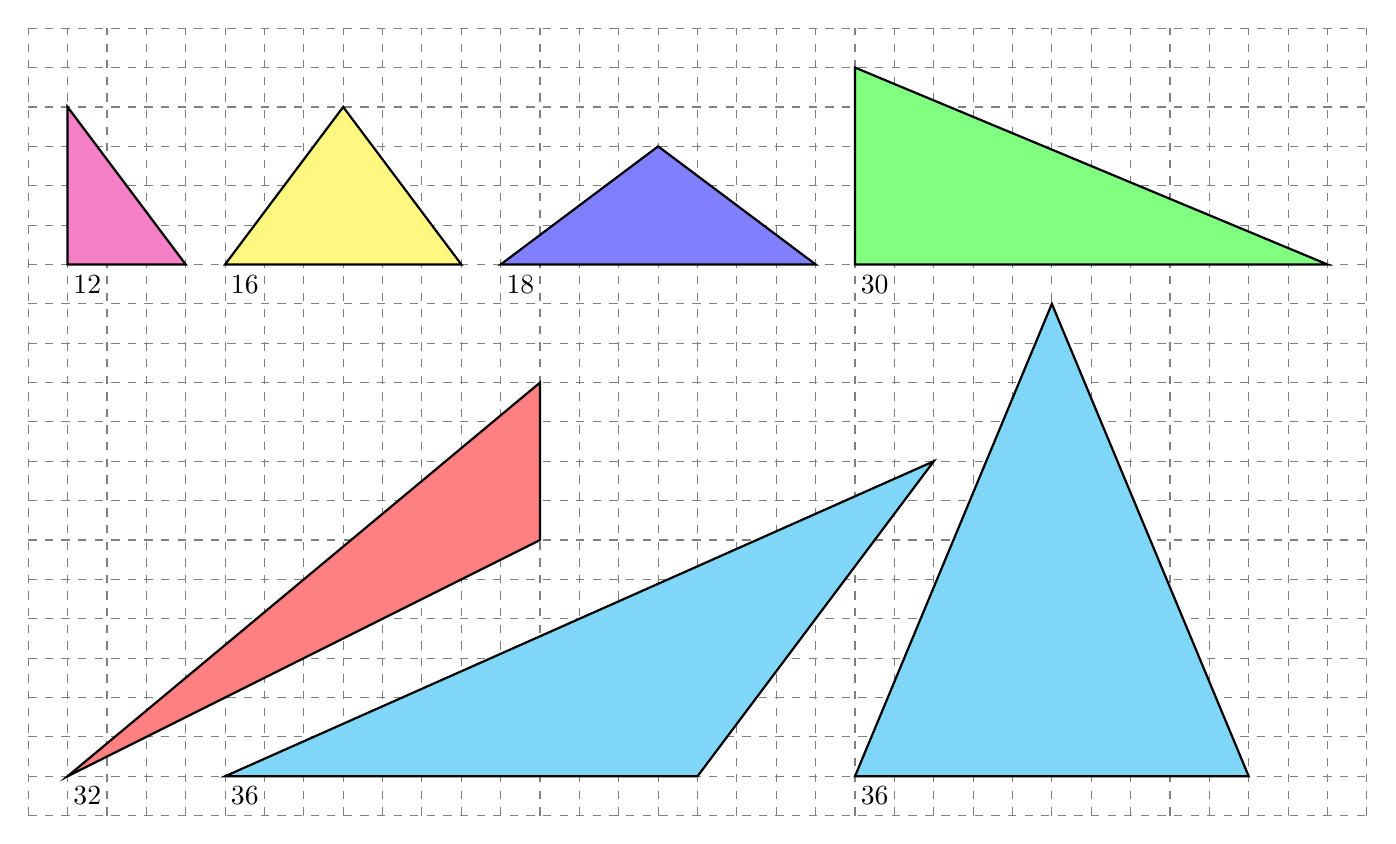
\begin{tikzpicture}[scale = 0.5]
    \draw[dashed, gray] (-1,-14) grid (33, 6);
    \draw[thick, fill=magenta!50] (0,0)--(0,4)--(3,0)--cycle;
    \node at (0.5, -0.5) {12};
    \draw[thick, fill=yellow!50] (4,0)--(10,0)--(7,4)--cycle;
    \node at (4.5, -0.5) {16};
    \draw[thick, fill=blue!50] (11,0)--(19,0)--(15,3)--cycle;
    \node at (11.5, -0.5) {18};
    \draw[thick, fill=green!50] (20,0)--(32,0)--(20,5)--cycle;
    \node at (20.5, -0.5) {30};
    \draw[thick, fill=red!50] (0,-13)--(12,-7)--(12,-3)--cycle;
    \node at (0.5, -13.5) {32};
    \draw[thick, fill=cyan!50] (4,-13)--(16,-13)--(22,-5)--cycle;
    \node at (4.5, -13.5) {36};
    \draw[thick, fill=cyan!50](20,-13)--(25,-1)--(30,-13)--cycle;
    \node at (20.5, -13.5) {36};
  \end{tikzpicture}
  \begin{tikzpicture}
  \end{tikzpicture}
  \begin{tikzpicture}
  \end{tikzpicture}
  \caption{
    The seven smallest primitive Heronian triangles as measured by perimeter.
  }
\end{figure}
\begin{question}
  Do Heronian $n$-simplices exist for all integers $n$?
\end{question}

\begin{related}
  \item Do infinitely many primitive Heronian $n$-simplices exist for each $n$?
  \item What is the smallest Heronian $n$-simplex for each $n$ as measured by
    volume? As measured by largest side? As measured by sum of sides?
    As measured by ``surface area'' (sum of volume of $(n-1)$-degree facets)?
  \item Are all Heronian $n$-simplices lattice simplices?
  \item What if the definition is relaxed so that only the volume and the
    edges must be integers?
\end{related}
\begin{references}
  \item \url{https://www.jstor.org/stable/2695390}
  \item \url{https://oeis.org/A272388}
  \item \url{https://en.wikipedia.org/wiki/Heronian_tetrahedron}
  \item \url{https://en.wikipedia.org/wiki/Simplex}
\end{references}
\end{document}
